% KEY TODOs:
%  * better title
%  * turn overview into combined overview and contribution
%  * Finish tool support section
%  *  -> reduce future work paragraph in conclusion accordingly

\documentclass[runningheads]{llncs}
\usepackage[show]{ed}
\usepackage{wrapfig}
\usepackage{xspace}
\usepackage{graphicx}
\usepackage{stex-logo}
\usepackage{paralist}
\usepackage{wrapfig}
\usepackage[hidelinks]{hyperref}
\usepackage{orcidlink}
%\usepackage{lststex} debug that the gray is not solid
\usepackage{listings}
\definecolor{codegray}{rgb}{0.9,0.9,0.9}
\lstset{basicstyle=\sf,columns=fullflexible,backgroundcolor = \color{codegray}}
\lstset{numberstyle=\tiny}
\lstset{language={[LaTeX]TeX}}
\usepackage[style=alphabetic,hyperref=auto,defernumbers=true,backend=bibtex,firstinits=true,maxbibnames=9,maxcitenames=3,isbn=false]{biblatex}
\addbibresource{kwarcpubs.bib}
\addbibresource{extpubs.bib}
\addbibresource{kwarccrossrefs.bib}
\addbibresource{extcrossrefs.bib}
\usepackage[noabbrev]{cleveref}
\usepackage{tikz}
\usetikzlibrary{shapes}
\usetikzlibrary{arrows}
\usetikzlibrary{docicon}

% I do not want to annotate just yet.

\newcommand\ALeA{\textsf{ALeA}\xspace}
\newcommand\SMGloM{\textsf{SMGloM}\xspace}
\newcommand\snify{\textsf{snify}\xspace}
\newcommand\defianno{\textsf{defianno}\xspace}
\def\llangle{\langle\kern-.2em\langle}
\def\rrangle{\rangle\kern-.2em\rangle}

\title{
    % Semantic Authoring in the \sTeX/\ALeA World
    % \ednote{Find better title. Was ``Bulk Semantic Annotation with a Partially Known Knowledge Base''}
Semantic authoring in a flexiformal context --- Bulk annotation of rigorous documents
}
\author{Michael Kohlhase\orcidlink{0000-0002-9859-6337} \and Jan Frederik Schaefer\orcidlink{0000-0003-2545-4626}}

% \keywords{semantic authoring, \snify, \sTeX, \ALeA, flexiformal content commons}
\institute{Computer Science, FAU Erlangen N\"urnberg, Germany}
\begin{document}
\maketitle
\begin{abstract}
%   Semantic annotations can be utilized for learning support services in technical
%   documents. The resulting active documents support more direct and personalized
%   interaction with the knowledge conveyed, but require a large investment in the authoring
%   process.
% 
%   In this paper we discuss the nature of the semantic authoring problem and argue that
%   while sharing aspects of classical, informal authoring and formal authoring, it is a
%   problem of its own that needs special editing support facilities. We present a simple
%   utility that supports the process of annotating technical terms with semantic references
%   to a flexiformal content commons that enhances annotation productivity by almost an
%   order of magnitude.

  Semantic annotations enable services that make the knowledge in documents more
  accessible.  In the case of \ALeA, a learning assistant we use as a case study, they
  enable, for example, guided tours and practice problems tailored to the learner's
  competencies.  However, the cost of semantic authoring is substantial and tool support
  is limited.

  In this paper we discuss the nature of the semantic authoring problem and argue that,
  while sharing aspects of classical (informal) authoring and formal authoring, it is a
  problem of its own that needs special editing support facilities.  We present and
  evaluate a simple utility that supports the process of annotating technical terms with
  semantic references to a flexiformal content commons that enhances annotation
  productivity by almost an order of magnitude.
\end{abstract}
% \setcounter{tocdepth}{3}
% \tableofcontents

\section{Introduction}
Arguably, dealing with large document collections is one of the key factors in the knowledge-driven society and economy.
There are currently two main contenders for machine support in this area.
Symbolic/logic-based technologies and sub-symbolic/machine-learning-based AI, e.g.\ via LLMs or chatbots.
They have complementary strengths and challenges:
ML-based approaches can be trained on all data of the Internet, but face challenges in precision and explainability. 
Symbolic technologies, on the other hand, offer precision and explainability out of the box, but face scalability challenges
-- in particular because of the cost of semantic authoring, which we discuss in this paper.

As a case study, we will use adaptive learning assistants for STEM subjects in higher education, concretely the \ALeA system \cite{BerBetChu:lssmkm23}.
We contend that machine-learning based technologies are largely unsuitable for this task -- at least until they reach the
precision and explainability required by the ethics of teaching --
while the scope of specific domains is just narrow enough that symbolic approaches are viable.
Conventional (\LaTeX-based) lecture materials can essentially be directly imported into \ALeA,
but its ability to generate learner-adaptive learning objects -- instrumented with learning support interactions --
depends on semantic annotations.
These can be embedded \LaTeX\ documents using the \sTeX package~\cite{MueKo:sdstex22,sTeX:github:on}.
In this paper, we will mostly focus on annotating terms with the semantic concepts they refer to,
but \sTeX supports a much wider range of annotations, such as annotating problems with the learning objectives
or annotating the defining phrase (definiens) in concept definitions,
and could, in principle, even be used for full formalization.
As \sTeX supports the spectrum from informal (un-annotated) to fully formalized content,
we say that \sTeX content is \textbf{flexiformal}.

The \textbf{\sTeX/\ALeA content commons} consists of \SMGloM~\cite{GinIanJuc:spsttom16},
a glossary acting as the domain model for semantic annotations,
as well as re-usable lecture materials such as lecture slides and problems.
% -- mostly from the area of computer science.
The sheer size
of the commons is one of the key challenges for authors: \SMGloM contains definitions of over
5400 concepts in multiple languages, created and maintained by over 30
contributors.  Additionally, there are roughly 4900
semantically annotated lecture slides and 4000 problems
-- mostly from the area of computer science.
% grep -R --include='*.tex' -F -e '\begin{frame}' | wc -l

% \ednote{
%     \textbf{Related work: semantic web authoring}
%     \emph{semantic authoring} already used in context of semantic web (RDFa).
%     Tools exist and it doesn't have exactly the same challenges as we face, though there is some overlap.
%     We have a module system and need more dependency management, something else?
%     This has to be described somewhere.
% 
%     Related work: ``User Interfaces for Semantic Authoring of Textual Content: A Systematic Literature Review.''
% }

\paragraph{Overview \& Contribution}
In this paper, we argue that semantic/flexiformal authoring shares aspects with both informal and fully formal authoring,
but is nevertheless a distinct problem requiring special tool support (\cref{sec:semauth}).
Using \sTeX/\ALeA as an exemplary case study,
we will provide an overview of the authoring support (\cref{sec:tools})
and then describe and evaluate one new, concrete tool, \snify, that supports the annotation
of terms with the semantic concepts they refer to (\cref{sec:snify,sec:eval}).
The paper ends with a brief conclusion (\cref{sec:conclusion}).


\paragraph{Acknowledgments}
The work reported in this article was conducted as part of the VoLL-KI project (see
\url{https://voll-ki.de}) funded by the German Research/Education Ministry under grant
16DHBKI089.

\section{Semantic Authoring in a Content Commons}\label{sec:semauth}

Before we discuss semantic authoring in general, let us introduce a concrete example from
the \sTeX/\ALeA world. We will use it to sharpen our intuitions of the challenges
involved and to ground the solution we propose.

\subsection{Running Example: Annotating ``terminal''}
With \sTeX, authors can add semantic references to technical terms,
which enables straight-forward learning support services like
showing the definition of a term, but also informs the system
about the content/prerequisites of a learning object.
Adding these references is a key practical problem when converting presentational {\LaTeX}
course materials into semantic documents.

\begin{figure}[ht]\centering
  \fbox{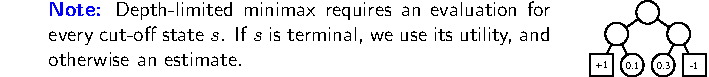
\includegraphics[width=10cm]{../img/minimax-remarks.pdf}}
  \caption{An annotated learning object from an AI lecture}\label{fig:lo}
\end{figure}

Take for instance a learning object like the paragraph in \cref{fig:lo}, where we want to annotate
the term ``terminal'' with the (semantic) concept of ``a goal state of a search
problem''. The latter can either be defined earlier in the course or in the domain model
(or both).

Concretely this is about converting the {\LaTeX} string
    (for conciseness completely unannotated)
    \ednote{MK: There is/was a discrepancy
  in the last line of the example; I tried to fix it, but failed\\
    FS: Is it fixed now? I don't see any discrepancy.}
\begin{lstlisting}[numbers=left,firstnumber=3,
caption=The unannotated {\LaTeX} sources of \cref{fig:lo},label=lst:los]
\item \blue{Note:} Depth-limited minimax requires an evaluation for every
cut-off state $s$. If $s$ is terminal, we use its utility,
and otherwise an estimate.
\end{lstlisting}
into the partially annotated item:
\begin{lstlisting}[morekeywords={sr,importmodule},numbers=left,
caption=Annotating ``terminal'' in \cref{lst:los},label=lst:losa]
\importmodule[smglom/search]{mod?search-problem}
[...]
\item \blue{Note:} Depth-limited minimax requires an evaluation for every
cut-off state $s$. If $s$ is \sr{goal state}{terminal}, we use its utility,
and otherwise an estimate.
\end{lstlisting}
In the latter, the author has the word ``terminal'' with the concept it refers to with 
via the \sTeX macro
\lstinline[mathescape]|\sr{$\llangle URI \rrangle$}{$\llangle verbalization\rrangle$}|.

\begin{newpart}{MK: more definitions}
  In \sTeX, objects and concepts are represented by \textbf{symbols}, which are identified
globally and unambiguously by a URI that includes a \textbf{namespace}, a \textbf{module
  name}, and a \textbf{symbol name}. Every symbol can have one or more
\textbf{verbalizations}:
words of the domain jargon used to refer to the concept or object.
Verbalizations can vary between between subdomains and communities of practice. In
our example, the verbalization ``terminal [state]'' was annotated with the symbol with
name \lstinline|goal state|. It comes from the module with name \lstinline|search-problem|
in the namespace \lstinline|smglom/search/mod| imported via the \lstinline|\importmodule|
macro in line 1. As the symbol name \lstinline|goal state| is unique in the imports here
it suffices as a relative URI in the \lstinline|\sr| annotation.

If the symbol name and the desired verbalization coincide (as they often do in English),
the short-hand macro \lstinline|\sn| can be used (e.g. as \lstinline|\sn{utility}| for ``utility'' in \cref{lst:losa}).\ednote{
    FS: Do we need the last paragraph?
        I've removed the ``sn utility'' annotation from the listing
        because I thought it breaks the flow a bit.
        But if we want to show the sn macro, I can add it back.
}
\end{newpart}

The annotation refers to a definition in the domain model module shown in
\cref{fig:state-space}.  The \lstinline|\definame| and \lstinline|\definiendum| in lines
5--6 introduce the verbalizations ``goal state'' and ``terminal state'' for the symbol
\lstinline|search-problem?goal state| introduced by \lstinline|\symdecl*| declaration in
line 3.

\begin{figure}[ht]\centering
  \fbox{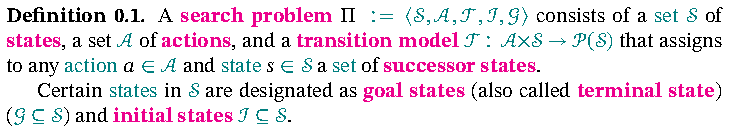
\includegraphics[width=12cm]{../img/search-problem.en.pdf}}
\begin{lstlisting}[morekeywords={definame,symdecl,definiendum},numbers=left,
escapechar=!]
\begin{smodule}[title=Search Problem]{search-problem}
[... some imports ...]
\symdecl*{goal state}
\begin{sdefinition}
  [...] Certain \sns{state} are [...] \definame[post=s]{goal state} [...]
  (also called \definiendum{goal state}{terminal states}).
\end{sdefinition}
\end{smodule}
\end{lstlisting}
  \caption{Simplified definition of ``goal state'' from the domain model}\label{fig:state-space}
\end{figure}

\subsection{Annotation Workflows and Requirements}\label{sec:workflows}

To annotate the word ``terminal'' in the document, the author has to be aware that it is a
technical term, that the module from \cref{fig:state-space} exists, know the symbol URI,
and manage redundancy of the imports -- i.e. only adding the \lstinline|\importmodule|
directive if it is not already (recursively) implied and possibly removing directives that
become redundant by the new one.  At ca 150,000 words in a semester's worth of lecture
notes and ca. 10--15\% of technical terms a rather daunting task.

While annotation needs to happen during authoring and curation of documents, the majority
of annotation tasks in practice concern the semantic augmentation of existing documents
(\textbf{bulk annotation}) with respect to an existing semantic domain model. In any case,
it is probably useful to separate the roles of author and semantic annotator conceptually,
even though they may well be the same person in practice.

The most important resource for annotators is a verbalization to symbol URI mapping -- we
call it the \textbf{annotation catalog} -- either implicitly in the mind of the annotator
or explicitly as a technical artifact, which allows to
\begin{inparaenum}[\em i\rm)]
\item identify the known technical terms,
\item to map them to the corresponding symbols, and 
\item manage the necessary import directives.
\end{inparaenum}
This catalog can be harvested from the \textbf{formal declarations}
(\lstinline|\definiendum|, \lstinline|\sr|, \lstinline[language={}]|\begin|/\lstinline[language={}]|\end{smodule}| and
\lstinline|\importmodule|, etc.) of the domain model and existing documents in the
semantic corpus.

In $L$-language documents, where $L$ is not English the annotation practices are a bit
more complex still, in particular because the annotation catalog is usually incomplete.

Note that for $L$-annotation, we need a $L$-specific annotation catalog. 
\sTeX already supports multilinguality:
\begin{itemize}
\item Documents have explicit language annotations (usually in form of the file extension
  \lstinline[mathescape]|.$\llangle lang\rrangle$.tex| where $\llangle lang\rrangle$ is the
  ISO-639 language identifier.)
\item Modules in the domain model allow $L$-translations that share the formal
  declarations with another module. In particular all definienda in $L$-modules are
  $L$-specific.
\end{itemize}

But still, $L$-annotation catalogs are usually inadequate for $L$-annotation tasks in
practice, as
\begin{enumerate}[\em i\rm)]
\item $L$-verbalizations and symbol names do not often coincide and
\item the domain model may not even have $L$-modules -- especially for the ``smaller''
  languages
\end{enumerate}
 In this situation, we usually have to invest in
establishing a suitable catalog e.g. by providing $L$-translations (or at least dictionary
information) in the domain model or delineating modules and annotating definienda that the
domain model does not cover in the documents to be annotated.
\ednote{FS: Todo: verbalizations can also be
inferred from existing annotations (without any $L$-modules).}

\subsection{Semantic Authoring as a Distinct Problem}
We contend that semantic authoring is a problem that is distinct from traditional
(informal) authoring and authoring fully formal corpora (e.g. programs or formalizations),
while sharing some of the aspects of either.

\paragraph{Traditional, informal authoring}
In traditional authoring e.g. of a scientific article or a textbook, the domain model -- a
highly structured model of the domain of discourse -- is in the authors' heads, and is
partially verbalized e.g. in the preliminaries section or the main sections of the
respective article. The content is informal -- usually a natural language like English
augmented with technical jargon, formulae, tables, and diagrams -- and designed for
processing via the brain of a colleague or student -- in any case, a human who shares a
canonical part of the domain model with the authors.\ednote{MK: this shared domain model
  could be thought of as the informal content commons; hmmm, but maybe the literature is
  the content commons} Consequently a large part of the authoring problem lies in
predicting the state and extent of the domain model of the reader and creating text that
bridges the gap between the reader's domain model and the payload content of the article
-- the knowledge the article or textbook intends to impart -- ideally using the technical
vocabulary the reader is familiar with to reduce this gap. Tool support for traditional
authoring is minimal and usually restricted to spell/grammar-checkers and online thesauri
if we disregard LLM-based writing/formulation support for now.

\paragraph{Formal Authoring}
In fully formal authoring e.g. for programming, the content commons is given formally in
the form of the libraries of the respective programming language, correspondingly the
authored content is also formal -- a program -- and intended for processing by a computer,
for which the formality is a prerequisite. Formal authoring is usually supported by an
integrated development environment (IDE) that makes use of the fully formal content and
offers services like semantic highlighting, tab completion, jumping to variable
declarations, function definitions, and interface definitions, as well as refactoring
support. All of these rely on a syntactic/semantic analysis of the formal content. The
situation is very similar for authoring of formal knowledge, e.g. in program verification
or the formalization of mathematics.

\paragraph{Semantic Authoring}
In semantic authoring, e.g. the \sTeX sources of educational content for the \ALeA system
presented above, the base of the text is classical narrative text to which most of the
constraints of classical authoring apply.
The exception is the tailoring to the competencies of the assumed reader
that traditionally happens during authoring, but which can (partially) be automated by systems like
\ALeA. Note that it is not a restriction that \ALeA is initially targeted to tertiary
education; the underlying mechanisms generalize to all scientific communication and
technical documents. After all, the purpose is to transfer information (instruct), even if
the roles of instructor and instructee are not predetermined by academic seniority.

But in addition to the base text, semantic authoring also has to provide the semantic
annotations that drive the personalization and interaction. Techniques from formal
authoring could help here, but in contrast to formal authoring, we cannot just trigger the
IDE functionality by the formal syntax, as the authored content is -- so far -- informal
and the content commons (the target of the annotations) is itself only flexiformal. In a
way, we need a local flexiformalization workflow that helps authors bridge the
informal-formal gap.

\paragraph{Semantic Authoring and the Semantic Web}
The phrase ``semantic authoring'' has also been used in the context of the semantic web with varying meanings.
This includes ontology authoring, which we would classify as formal authoring,
and metadata annotation (e.g. the title, author, and creation date of a document),
which is a somewhat different concern.
A closer match is the annotation of informal content with
references to a domain ontology,
but there are some differences to our situation with \sTeX/\ALeA:
The domain ontology would be a fully formal target
-- possibly containing verbalizations --
while in our case the target is flexiformal.
Furthermore, \sTeX has a module system, which requires
dependency management during authoring.

\section{Tool Support for Semantic Authoring in \sTeX/\ALeA}\label{sec:tools}

Semantic authoring can ``inherit'' tool support from both informal and formal authoring.
In the case of \sTeX, we can re-use spell checkers for traditional informal authoring.
There also is prototypical support for authoring \ALeA content in Microsoft Word with a
custom plugin (see \cite{KohKoh:woide24}), which allows authors to use Word's spell
checker and grammar checker.\ednote{MK: Mention CPoint and SMD as well? Probably yes.}

On the formal side, there is a custom VSCode IDE plugin for \sTeX \cite{sTeX-IDE:git} that
analyzes annotations on the fly, displays the underlying reference semantics, reports
errors and redundancies, and even offers a concept search interface.  But such features
only support existing annotations and are, therefore, of limited use when creating new
annotations, which arguably is the most time consuming aspects of semantic authoring.
% \ednote{also: SPARQL API}

How the annotation process can be supported depends on the particular semantic framework,
the specific annotations we want to support, and the semantics embedded in the content
commons.  In \sTeX/\ALeA, we primarily annotate formulae and technical terms with pointers
to their definienda.  A tool for supporting semantic authoring of formulae via notations
has been presented by Vre{\v{c}}ar et al.\ in~\cite{VreWelKam:tsmmdui24}.  It uses a
grammar to parse informal, presentation-focused formulae (e.g.\
\lstinline[keywordstyle={}]|A\times B|) into abstract syntax trees based on semantic
macros defined in \sTeX, which can then replace the original formula (e.g.\
\lstinline|\cart{A,B}| for the Cartesian product of sets).  In the case of ambiguity,
authors can pick the correct reading in a graphical user interface that visualizes the
different abstract syntax trees.

Efficient support for the annotation of technical terms in natural language
has been elusive so far.


\section{The \snify System}\label{sec:snify}

The \snify\footnote{ From ``\texttt{\textbackslash sn}-ify''; ``\texttt{\textbackslash
    sn}'' is a frequently used \sTeX short-hand macro for term annotations.}  utility
\cite{stextools:git} is a simple command-line tool that creates a catalog of
symbol-verbalization pairs, analyzes \sTeX source files, and then steps through all word
occurrences in the document that match a verbalization in the catalog.  Matching is based
on word stems using off-the-shelf stemmers, which allows us to e.g.\ match ``utilities''
with ``utility''.  For each matched word, the user is presented with an annotation choice
and interactions that allow to fine-tune the wordwise annotation workflow.  The interface
is inspired by traditional spell checkers like \lstinline|ispell|.  \Cref{fig:snify} shows
a typical situation.

\begin{figure}[ht]
  \setlength{\fboxsep}{0pt}
  \fbox{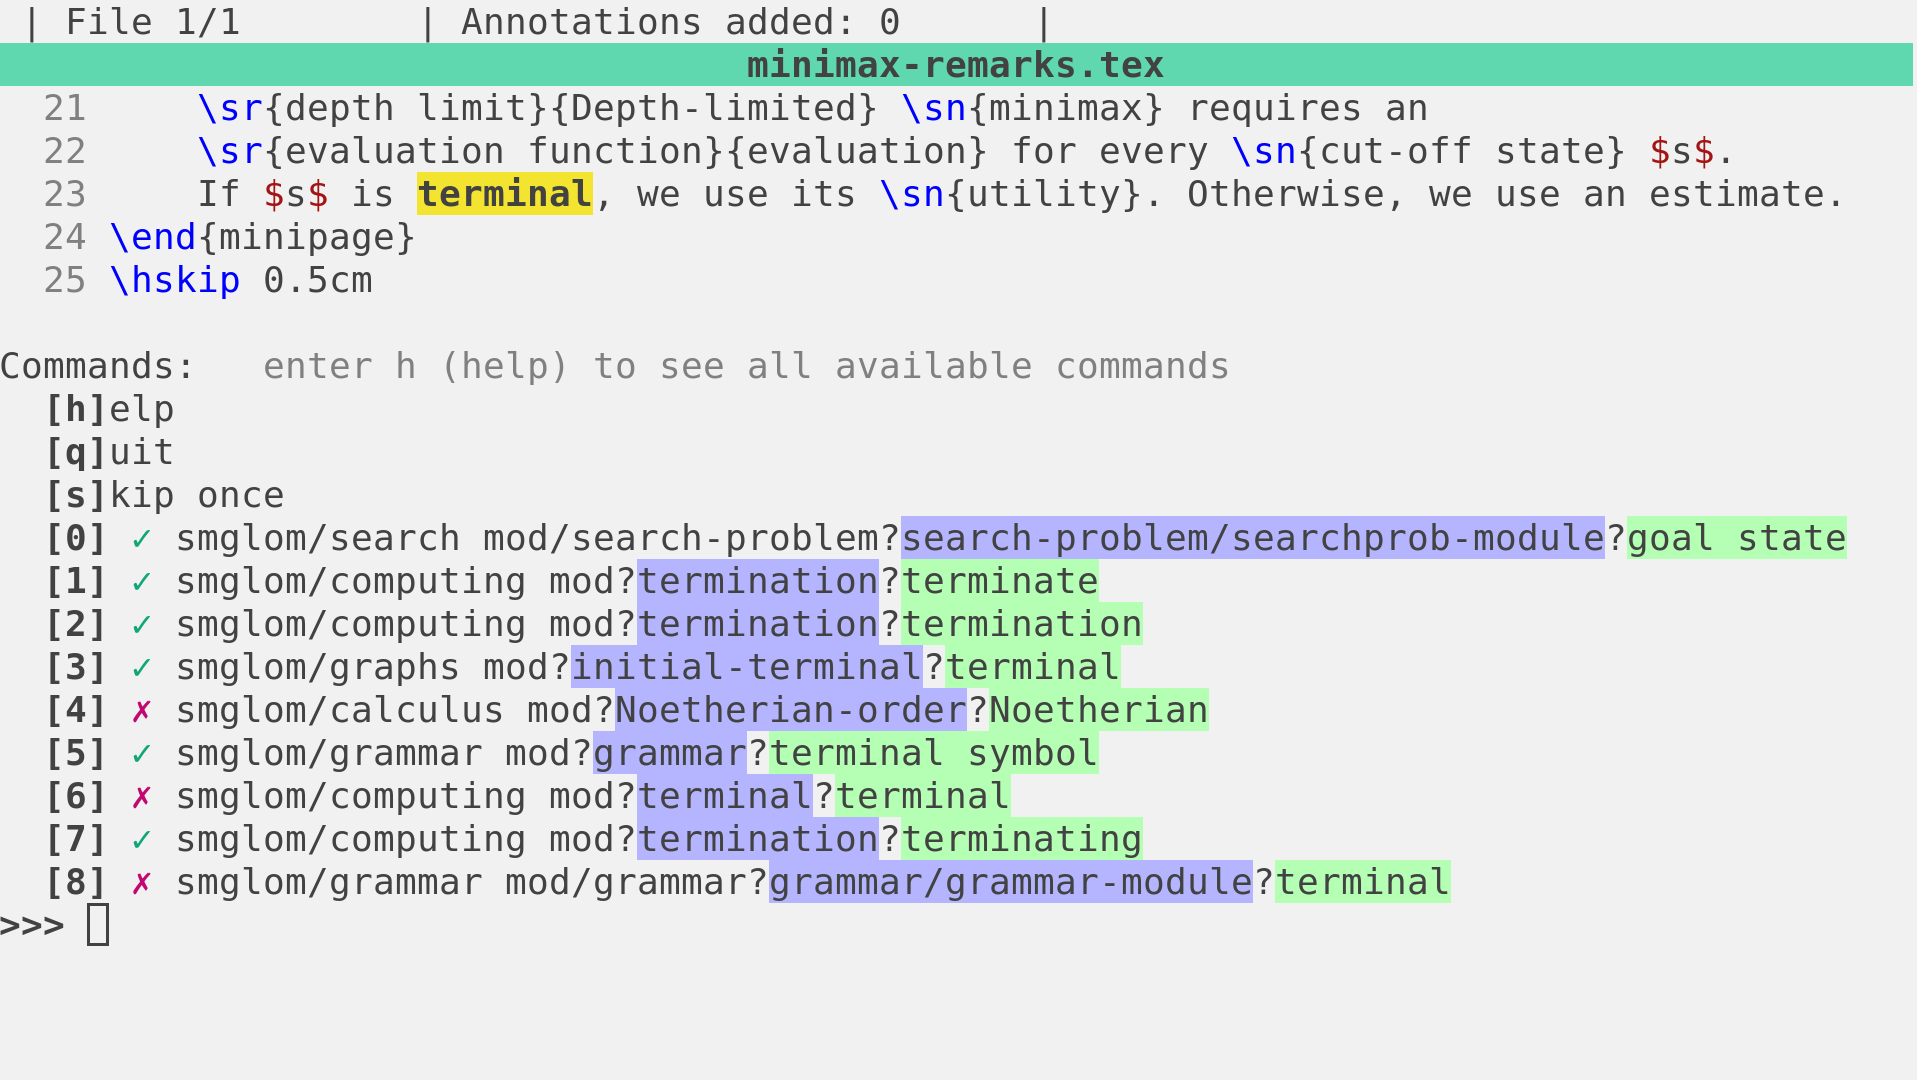
\includegraphics[width=12cm,trim={0 3cm 0 0},clip]{../img/snify}}
  \caption{\snify in Action: Annotating the word ``terminal''.}\label{fig:snify}
\end{figure}

The annotator can choose an annotation by typing the corresponding choice number,
in this case \lstinline|0|.
The little green check-mark indicates that the relevant module is already imported.
Otherwise \snify would offer the annotator the choice to import it -- if we are
in a module context -- or to add a \lstinline|\usemodule| directive, either in the
local environment or at the top-level.

To skip the word, the user can type \lstinline|s|,
\lstinline|s!| skips it until the end of the file, and \lstinline|S|
will skip it in future runs as well by appending a comment to the file.
There are numerous other commands, e.g.\ to adjust the selection,
search for alternative annotation targets,
or view/edit the file introducing one of the choices.

\snify is usually called on a set of files -- e.g. in a directory or math archive -- which
together form a \textbf{session}, which can be interrupted and resumed without having to
re-do all the \lstinline|s| skips. Alternatively, \snify can be called e.g. on the
top-level lecture notes; then the session consists of all (transitively) included
files. Other productivity features include a focus mode that can be used to only annotate
a particular word in the rest of the file, session, or the whole \sTeX/\ALeA corpus before
resuming regular annotation. This reduces the cognitive overhead from switching between
different words and symbol lists.
% Of course the include management still needs to be done locally.

\paragraph{Definition Handling as a Pre-process for Multilingual Documents}
As a companion to \snify, we have \defianno, a prototype tool for annotating definienda in
documents that were originally authored without semantic annotations.  It can be
configured to use different \LaTeX\ macros to identify definienda (e.g.\ \lstinline|\emph|
or \lstinline|\textbf|), and then steps through them similarly to \snify.  For each
potential definiendum, the user can then use fuzzy search to find the corresponding symbol
in the domain model.  This populates the catalog with verbalizations relevant to the
document, making subsequent \snify runs more effective, especially for documents in
languages that are not well covered by the domain model (i.e.\ not English).

\begin{newpart}{MK: rewritten as existing but experimental. This needs to be placed
    somewhere else.}
  \paragraph{Scaling \snify to the Flexiformal Content Commons }
One practical problem with \snify system as presented so far is that it only harvests
symbol/verbalization pairs from \sTeX files on the local file system. This means that, for
effective annotation, users (have to) download the whole content commons and keep it
updated -- an assumption/requirement that becomes increasingly impractical as the \sTeX
ecosystem grows.

The general situation is that on the one hand there is a constantly growing, shared
\textbf{content commons} of public math archives -- currently 200 with about 14.000 \sTeX
files -- that are regularly converted to FTML (\underline{F}lexiformal \underline{T}ext
\underline{M}arkup \underline{L}anguage) and served on \url{https://MathHub.info}. On the
other hand authors are working on
\begin{compactenum}[\em i\rm)]
\item a set of local working copies of the archives -- with the intention of publishing
  them on MathHub.info and their dependencies (they need to be local, since pdflatex
  cannot deal with remote files) and
\item possibly a set of private archive (think papers under development or exam
  problems/solutions) 
\end{compactenum}
This situation is familiar from software development and also from e.g. the \LaTeX
ecosystem. Semantic authoring -- and thus the \snify utility -- inherits the requirements
from both.

\begin{wrapfigure}r{5.5cm}\vspace*{-2em}
  \begin{tikzpicture}[scale=.7]
    \tikzstyle{doc}=[draw,thick,align=center,color=black,
                  shape=document,minimum width=10mm,minimum height=15mm]
    \tikzstyle{database}=[cylinder,shape border rotate=90,aspect=0.25,draw, 
     cylinder uses custom fill,cylinder body fill=yellow!30,cylinder end fill=yellow!30]
     \tikzstyle{include}=[right hook-angle 45,thick]
     \tikzstyle{includeleft}=[left hook-angle 45,thick]
    \node[doc] (cc) at (0,-1) {\shortstack{Content\\ Commons}};
    \node[doc] (pl) at (5,-1) {\shortstack{Private/\\Local}};
    \node[database] (db) at (3,2.5) {\shortstack{\tiny Verbalization\\Cache}};
    \node[draw] (sn) at (0,4.5) {\snify};
    \node[draw] (id) at (2.5,5) {IDE};
    \node[draw] (wo) at (5,4.5) {WOIDE};
    \draw[draw,fill=black!10] (-1.3,.5) rectangle ++ (6.4,1); 
    \node (f) at (-.5,.9) {\flams};
    \draw[include]  (cc) -- node[left] {\tiny F2RDF} (db);
    \draw[includeleft] (pl) -- node[right] {\tiny linter} (db);
    \draw[->] (db) -- (sn);
    \draw[->] (db) -- (id);
    \draw[->] (db) -- (wo);
    \draw[dashed,thick] (3,1.6)  -- (3,-2);
    \draw[dashed,thick] (3,1.6)  -- (3,-2);
    \draw[includeleft] (pl) to[bend right=10] (wo);
  \end{tikzpicture}
  \caption{Architecture}\label{fig:arch}\vspace*{-1em}
\end{wrapfigure}
To cope with this situation, We have extended the brand-new \flams system
\cite{flams:on}\footnote{A paper on \flams is submitted to CICM 2025 and will be cited
  here if accepted.} with functionality for handling definienda in the FTML2RDF harvester,
so that all symbol/verbalizations are available in the \flams triple-store. Thus a harvest
from the flexiformal content commons is just a simple SPARQL query and some postprocessing
of the result (de-duplication, stemming, and pairing) away. Note that \flams works
directly on FTML, which is generated from \sTeX input by \textsf{rus\TeX} and exported
from annoated MS Word files via WOIDE.

In local/private archives, the \snify harvester needs to work directly on the \sTeX
sources. Here we have extended the \flams \textbf{linter} -- a simple \sTeX parser that
drives the LSP functionality the VSCode and \texttt{emacs} \sTeX IDE plugins use to deal
with definienda. This is much more efficient (and robust) than the initial regex-based
python parser). The analogon for this on the WOIDE side is still under development it
could be based on FTML generated by WOIDE, or WOIDE could export symbol/verbalization
pairs into the \snify verbalization cache directly.

In this situation, the main functionality of \snify is to maintain the verbalization cache
and answer front-end queries for verbalizations efficiently so that we can power various
front-ends from that. These include
\begin{compactenum}[\em i\rm)]
\item The traditional text/terminal-based \snify UI for bulk annotation,
\item the \sTeX IDEs in VSCode and \texttt{emacs} that can supply while-editing annotation
  support, and 
\item WOIDE, which can be seen as a semantic authoring IDE based on MS Word.\ednote{MK:
    CPoint and semantic wikis.}
\end{compactenum}

Note that implemented this broadly \snify can provide additionall logistic services: If a
pair is chosen in an annotation, \snify can then automatically download the corresponding
archive so that the annotated file can be formatted with \texttt{pdflatex} or
\textsf{rus\TeX} locally.
\end{newpart}

\section{Practical Evaluation and Future Work}\label{sec:eval}
\begin{wrapfigure}{r}{0.4\textwidth}
  \centering
  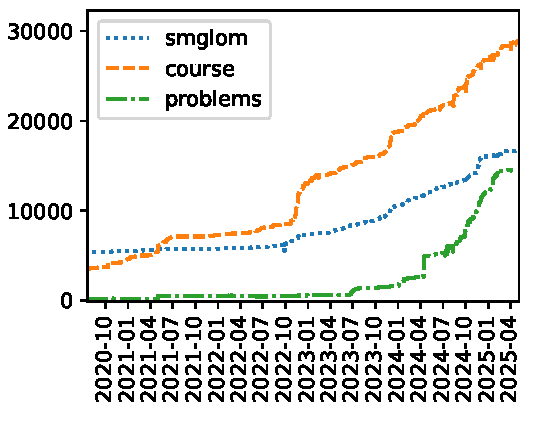
\includegraphics[width=0.4\textwidth]{../img/annocounts.pdf}
  \caption{Number of annotated terms in the \sTeX/\ALeA commons over time.}\label{fig:annocounts}
\end{wrapfigure}
In our experience, \snify's step-through workflow for annotating term references for symbols
from the domain model is almost an order of magnitude more efficient than writing the
annotations and imports by hand, even for annotators who are familiar with the domain
model.
Given the sheer number of term annotations (see \cref{fig:annocounts}),
this results in a considerable productivity gain.
For annotators unfamiliar with the domain model, the unassisted annotation task is
almost infeasible, and the average unfamiliarity naturally grows with the domain
model. The symbol disambiguation process -- on average a word induces 4.1 choices
% \ednote{
%     more details? median is 3, for existing annotations, the average is 2.6 and the median 2...
% }
-- is still manageable,
requires considerable concentration and domain knowledge, but little knowledge of the
domain model flexiformalization.

The command-line interface is simple and responsive and gives all the necessary
information in a single glance if the underlying shell area exceeds ca. $80\times 35$
characters. It is very much geared towards annotating existing documents with respect to a
relatively complete -- pre-existing -- domain model, and it seems unlikely that a more
sophisticated UI would add value for this use-case.

For less complete domain models we have to skip too many terms that should ultimately be
annotated and annotation efficiency suffers.\ednote{
    FS: Isn't this wrong? We don't have to skip them, the problem is that \snify skips them.
    Efficiency does not suffer, but rather effectiveness.
}
This is currently the case for all
non-English languages in the \sTeX corpus we work with. Coverage in German is only about
half of that of English and we can already see the practical effects.
The \defianno tool (see end of \cref{sec:snify}) can mitigate this partially by
providing verbalizations for the definienda in the document,
but we also want to annotate terms that are not explicitly defined in the document.
A potential solution would be to extend \snify with a machine learning-based
tool for identifying unannotated technical terms that are not in the catalog.
The user could then pick a symbol for annotation, which would add a verbalization to the catalog.
In an earlier (pre-\snify) attempt, we used named-entity
recognition (NER) for classification of ``likely annotation candidate words''
\cite{hutterer:msc23}. However, this classification was not precise enough in the
distinction in ``technical terms'' and ordinary English noun phrases
to be practical on its own.
A combination with \snify's catalog-based approach might change the trade-offs involved.


% For less complete domain models we have to skip too many terms that should ultimately be
% annotated and annotation efficiency suffers. This is currently the case for all
% non-English languages in the \sTeX corpus we work with. Coverage in German is only about
% half of that of English and we can already see the practical effects. We have also
% experimented with a Slovene introductory math book, and it seems clear that apart from
% having to introduce a Slovene stemmer\ednote{MK@FS: there is one for python at
%   \url{https://repo.ijs.si/pboskoski/slo_stemmer}}, we would need to manually annotate all
% definienda in the book before we can harvest the symbol/verbalization pairs which are a
% prerequisite for annotation.\ednote{this is in principle possible with \defianno}
% \ednote{don't even need definienda - sn annos are enough to populate the catalog}
% \ednote{TODO: I've commented out Hutter in conclusion - we can integrate it here as a potential workflow}


Finally, the current interface is not well-suited for on-the-fly annotation while
authoring.
For that, the underlying information (the symbol/verbalization pairs harvested
from the domain model) can be integrated into any IDE. In fact we plan to do this for the
next version of the sTeX plugin for VSCode \cite{sTeX-IDE:git}.
For now, the typical workflow of early adopters is to first write the document (e.g.\ a set of quiz questions) without annotations, and then run \snify to annotate the new content.

\section{Conclusion}\label{sec:conclusion}

In this paper we have presented the semantic authoring problem using the \sTeX corpus and
the adaptive learning assistant \ALeA as a concrete example. We have shown that it differs
from both classical authoring and formal authoring in terms of the necessary system
support. As an example of specialized authoring support, we have presented \snify, a
command-line tool that bridges the gap between informal text and formal symbols in \sTeX.

\snify is open source; the source and documentation are available from
\cite{stextools:git}.

% In an earlier attempt to support semantic annotation in IDEs, we tried named-entity
% recognition (NER) for classification of ``likely annotation candidate words''
% \cite{hutterer:msc23}, however this classification was not precise enough in the
% distinction in ``technical terms'' and ordinary English noun phrases and named entities --
% the relevant task for annotation, and so made it impractical, especially, since it could
% not enter the actual annotations and import directives automatically. But maybe using the
% NER-based approach, after the \snify annotation process might change the trade-offs
% involved. In any case, the overall workflow suggested by the NER-based approach --
% especially after the verbalizations covered by the existing domain model\ednote{introduce
%   in the definition above that the domain model is all definitions, not only in the
%   smglom?} -- is geared towards adding modules and symbols -- the ones discovered by NER
% -- to the domain model. 

\printbibliography
\end{document}

%%% Local Variables:
%%% mode: latex
%%% TeX-master: t
%%% End:

% LocalWords:  tbw Aarne Ranta homostem pre hmmm Vre ar al sn ify TODO et Hutter Plivelic
% LocalWords:  lang DHBKI FS Todo FTML lexiformal arkup anguage CICM RDF postprocessing
% LocalWords:  de
